\documentclass[10pt,twocolumn,letterpaper]{article}

\usepackage{cvpr}
\usepackage{times}
\usepackage{epsfig}
\usepackage{graphicx}
\usepackage{amsmath}
\usepackage{amssymb}
\usepackage{subcaption}
\usepackage{subfig}
\usepackage{algpseudocode}
\usepackage{float}

% Include other packages here, before hyperref.

% If you comment hyperref and then uncomment it, you should delete
% egpaper.aux before re-running latex.  (Or just hit 'q' on the first latex
% run, let it finish, and you should be clear).
\usepackage[breaklinks=true,bookmarks=false]{hyperref}

\cvprfinalcopy % *** Uncomment this line for the final submission

\def\cvprPaperID{****} % *** Enter the CVPR Paper ID here
\def\httilde{\mbox{\tt\raisebox{-.5ex}{\symbol{126}}}}

% Pages are numbered in submission mode, and unnumbered in camera-ready
%\ifcvprfinal\pagestyle{empty}\fi
\setcounter{page}{1}
\begin{document}

%%%%%%%%% TITLE
\title{Modeling and Packing Objects and Containers through Voxel Carving}

\author{Alex Adamson\\
{\tt\small aadamson@stanford.edu}
\and
Nikhil Lele \\
{\tt\small nlele@stanford.edu}
\and 
Maxwell Siegelman \\
{\tt\small maxsieg@stanford.edu}
}

\maketitle
%\thispagestyle{empty}

%%%%%%%%% ABSTRACT
\begin{abstract}
   This paper describes a system which attempts to determine whether it is possible to pack a set of objects into a container. This is done by using multiple photos of each object on a calibration grid to generate 3D models of the objects and containers plus a bin packing algorithm to find a working arrangement of the objects. We found that by using the CIELab colorspace it was possible to use K-Means clustering to reliably silhouette many pictures of the object with minimal user interaction, which allowed for the creation of reasonably accurate voxel models through carving. We also found that the number of frames used for each object impacted the size of the voxel models and the efficiency of the bin packing algorithm. More frames made the number of voxels in the objects decrease and thus allowed more of them to be packed. It also decreased the number of voxels in the container, which decreased the number of objects that the algorithm said could be packed. 
\end{abstract}

%------------------------INTRODUCTION
%-------------------------------------------------------------------------

%%%%%%%%% BODY TEXT
\section{Introduction}

We create a semi-supervised system to create 3D models from photographed objects and containers, and then determine how to fit the objects in the containers. For example, one could take pictures of toys and pictures of a box and the system would determine if those toys could be fit into the box. Our method relies on determining the pose of the camera (camera parameters), silhouetting the object from the background, creating a 3D model from the photos, and determining the way to pack the objects.

\subsection{Review of Previous Work}

Previous work in image segmentation and silhouettes use a variety of different methods. For example, there are simple threshold methods, clustering methods using K-Means, EM, and mean shift \cite{comaniciu2002mean} \cite{liureview}, the watershed method \cite{beucher1992morphological}, and graph based methods such as normalized cut \cite{shi2000normalized}.

There are a number of methods to do 3D model generation from views. These include space carving for voxel models \cite{kutulakos2000theory} and mesh acquisition from stereo imagery \cite{morency2002fast}.

Bin packing is a problem with implications for a variety of industries, so a number of heuristics exist. The heuristic we chose to base our algorithm on moved from the bottom of the container to the top, creating levels and trying to fill each level with objects of the appropriate size \cite{bialek2014packaging}.

We were also inspired by the project from March 2014: ``Counting jelly beans: voxel carving and segmentation of a container of heterogeneous objects.'' \cite{jellybeans}


\subsection{Key Contributions}
Our first key contribution is showing that a system combining silhouetting, voxel carving and a packing heuristic with minimal supervision can output reasonable estimates for how many objects can be packed into a container as well as arrangements of a variety of objects in a container. An important sub-point of this contribution is the usage of k-means along with the CIELab colorspace and minimal human interaction in order to quickly form silhouettes from input photos. Another key contribution from this paper is the investigation of how the number of frames used as input effects the results of the process, specifically the bin packing efficiency.

%------------------------------- Technical solution ----------------------------------------
\section{Technical Solution}

\subsection{Determining Camera Pose}

In order to extract the camera extrinsics for each viewpoint around an object and to get the camera intrinsics, we use Matlab's camera calibration toolbox and then transform the parameters so that we can left-multiply world coordinates by the projection matrix in order to recover image points. This necessitates having the camera calibration grid in each picture. The camera calibration toolbox assumes that we are right-multiplying:
\begin{align*}
    x^T &=  X^T P^T \\
    &= X^T \begin{bmatrix} R^T \\ T^T \end{bmatrix} K^T
\end{align*}
so in order to be able to recover image points via left-multiplication, we simply take the transpose of all the component matrices:
\begin{align*}
    x^T &= X^T \begin{bmatrix} R^T \\ T^T \end{bmatrix} K^T \\
    \Rightarrow x &= (X^T \begin{bmatrix} R^T \\ T^T \end{bmatrix} K^T)^T \\
    &= K \begin{bmatrix} R & T \end{bmatrix} X
\end{align*}
\subsection{Silhouette Generation}

Our method to mask out the silhouette of the object relies on having a contrasting color with the background. We use the K-Means algorithm, which iteratively partitions data by assigning every data point to one of $K$ clusters, where $K$ is chosen before hand. In our case, the data points are every pixel in the image, and the clusters correspond to the most prominent colors in the image.

To mask out the silhouette of the object, we select all pixels that correspond to a particular cluster chosen by the user. For example, for a blue bowl we select the pixels from the cluster with the most blue centroid. See figure \ref{bowl-kmeans-clusterids} where each pixel is colored black, gray, or white corresponding to which cluster it has been assigned to. Then in figure \ref{bowl-kmeans-silhouette} we mask out only the pixels from the most blue centroid. Note: We choose a low value of $K$ such as 3 or 4 to ensure that we end up with a conservative estimate of the silhouette that will later be carved down by other views.

Lastly we refine the mask by morphologically closing the holes in the image with circles of a small radius. We use the Matlab $\texttt{imclose}$ function, which uses methods based on morphological reconstruction \cite{soille2013morphological}. See figure \ref{bowl-kmeans-infill}.

\begin{figure}[ht]
    \centering
    \begin{subfigure}[t]{0.2\textwidth}
        \centering
        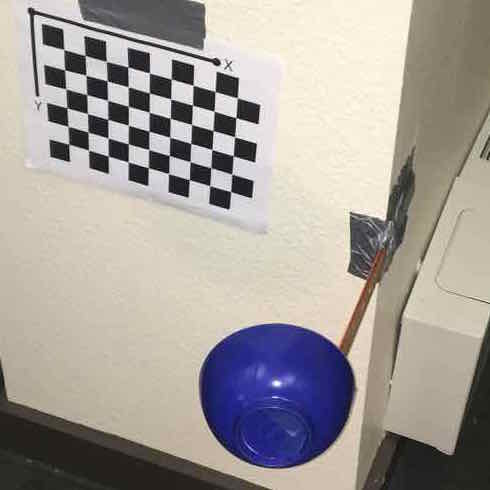
\includegraphics[width=\textwidth]{bluebowl_5.jpg}
        \caption{Original photo of blue bowl}
    \end{subfigure}
    ~ 
    \begin{subfigure}[t]{0.2\textwidth}
        \centering
        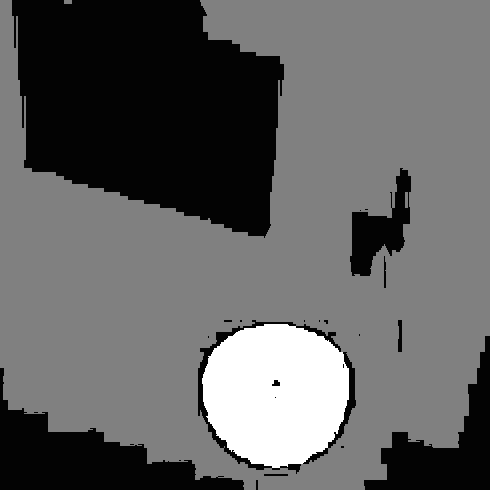
\includegraphics[width=\textwidth]{cluster_ids.png}
        \caption{Color-coding of clusters}
        \label{bowl-kmeans-clusterids}
    \end{subfigure}
    ~\\
    \begin{subfigure}[t]{0.2\textwidth}
        \centering
        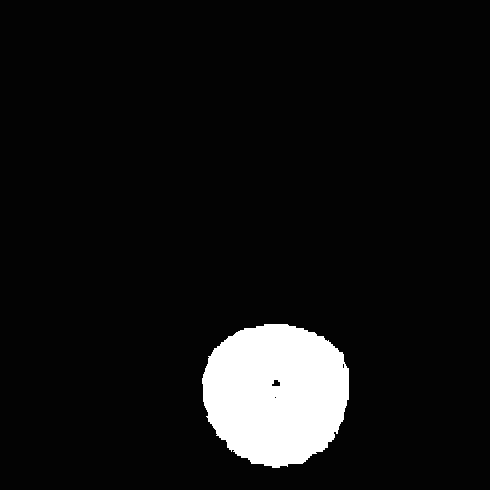
\includegraphics[width=\textwidth]{silhouette.png}
        \caption{Mask of just the blue bowl}
        \label{bowl-kmeans-silhouette}
    \end{subfigure}
    ~
    \begin{subfigure}[t]{0.2\textwidth}
        \centering
        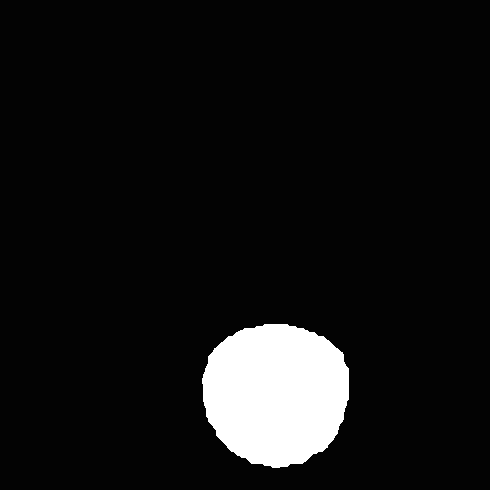
\includegraphics[width=\textwidth]{silhouette_infill.png}
        \caption{Refining mask with infilling}
        \label{bowl-kmeans-infill}
    \end{subfigure}
    \caption{Pipeline for silhouette acquisition using K-Means and infilling.}
    \label{bowl-kmeans}
\end{figure}

\subsubsection{CIELab Color-Space}

Before finding the silhouette, we first convert the image from RGB color-space to the CIELab color-space. The CIELab color-space consists of a lightness axis `L' and two color channels `a' and `b'. The `a' channel runs from green to red and the `b' channel runs from blue to yellow \cite{AdobeCIELAB}. See figure \ref{cielab} for a visualization of the axes of the color-space. This color-space is more useful for separating images on the basis of color because it more faithfully represents the way humans see color at the expense of not corresponding to pixels on our screens. Grays, browns, and other dull colors are harder to reason about in CIELab because they all lie near the origin, but our example objects have stronger colors that are especially suited to this color-space. In addition, because the lightness value is orthogonal to the color information, we can choose to only use the color axes for K-Means. This makes the clustering robust to changes in lighting and shadows.

\begin{figure}[H]
    \centering
    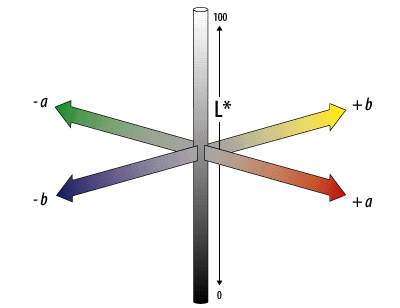
\includegraphics[width=0.4\textwidth]{CIELAB.png}
    \caption{Axes of the CIELab color-space \cite{AdobeCIELAB}}
    \label{cielab}
\end{figure}

In figure \ref{bowl-lab-rgb} we can clearly see that in RGB space and with the full CIELab space that the blue bowl is in the same cluster as parts of the checkerboard and the wall-mounting apparatus. By removing the lightness value and only considering the color channels `a' and `b', we are able to easily separate the blue bowl from the background and distinguish it from the other items in the picture.

\begin{figure*}
    \centering
    \begin{subfigure}[t]{0.2\textwidth}
        \centering
        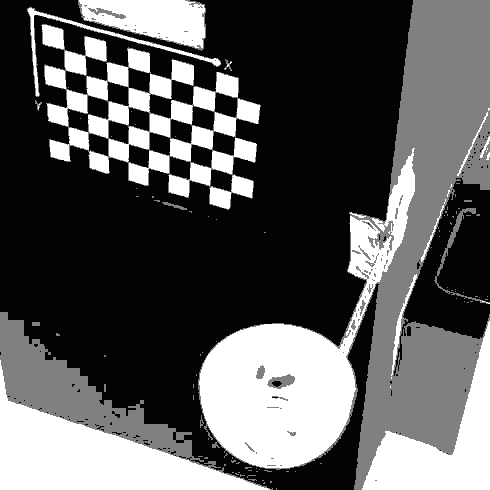
\includegraphics[width=\textwidth]{cluster_ids_RGB.png}
        \caption{K-Means in RGB space}
    \end{subfigure}
    ~ 
    \begin{subfigure}[t]{0.2\textwidth}
        \centering
        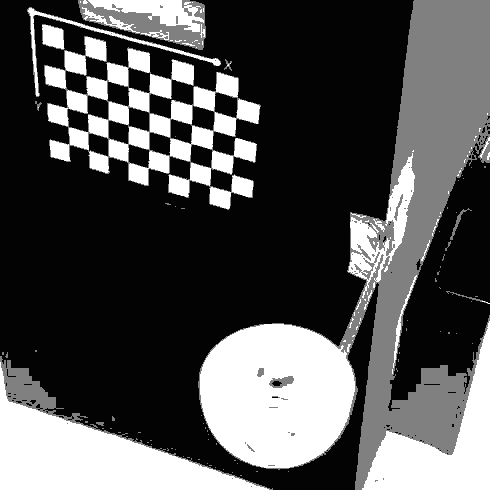
\includegraphics[width=\textwidth]{cluster_ids_full-lab.png}
        \caption{K-Means using full CIELab space}
    \end{subfigure}
    ~ 
    \begin{subfigure}[t]{0.2\textwidth}
        \centering
        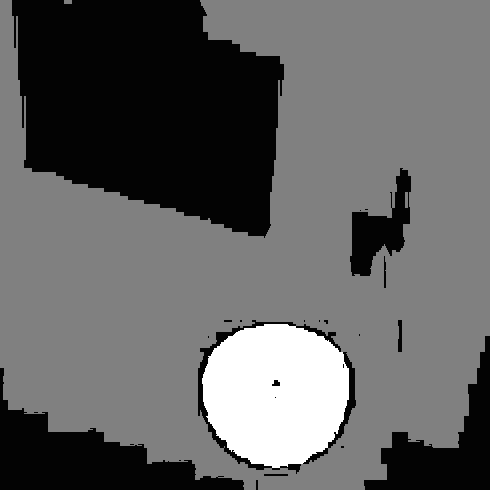
\includegraphics[width=\textwidth]{cluster_ids.png}
        \caption{K-Means without lightness from CIELab space}
    \end{subfigure}
    \caption{Comparing silhouette quality using different color-spaces. K-Means using only the color channels from CIELab space performs much better than either using RGB space or using the full CIELab space.}
    \label{bowl-lab-rgb}
\end{figure*}


\subsection{3D Model Generation}

For 3D model generation, we use a standard voxel carving approach. Given a set of tuples $F$ where $F_i = (P_i, S_i, I_i)$ containing the camera projection matrix $P_i$, the silhouette of the object $S_i$ in the image, and the image from the $i$th viewpoint $I_i$, we form a voxel model for the object as follows: Using the camera parameters and silhouette of the first tuple (here we assume that all images contain the entire object within their frame), we construct an initial bounding voxel prism. On successive iterations, for each voxel that has not been cut out yet, we remove it from the carving either if it projects outside of the frame of the image (since we are assuming that for each image, the entire object is contained in the frame) or if it projects into a pixel in the silhouette that was not considered part of the object by the silhouette-forming algorithm.

\begin{algorithmic}
\Function{Carve}{$c, P, S, I$} \\
    \State $X \gets P * c$
    \State $packings \gets 0$
    \For {$X_i \in X$}
        \If{$S(X_i) = 0$}
            \State $c \mathrel{-}= c_i$
        \EndIf
        \If{$X_i \notin I$}
            \State $c \mathrel{-}= c_i$
        \EndIf
    \EndFor
    
    \State \Return $c$
\EndFunction
\end{algorithmic}

Our use of a straightforward voxel carving algorithm is justified by the fact that we are assuming that our containers are hollow and hence we in general do not care about concavities since they will not affect how many objects we can place in them later in the pipeline. Additionally, our bin packing algorithm is not advanced enough to allow objects within the container to interlock within each other's concavities, so there is no potential gain from the perspective of getting more efficient packings (less approximation error) by improving the carving routine.

\subsection{Bounding Boxes}

It greatly simplified the bin packing algorithm to put the object models in bounding cuboids rather than trying to pack them immediately. While algorithms exist which find the smallest bounding box of an object using the convex hull of the object's point cloud, we decided it would be prudent to save time on this aspect and simply bound the voxel model by its smallest and largest x, y and z coordinates. This approach results in some inefficiency, both because a bounding box is strictly larger than the object it bounds and because the boxes we chose to use were not minimal, but it provides sufficiently good performance to allow us to examine the viability of our overall setup as well as how changing our silhouetting algorithms and their inputs affects the efficiency of our bin-packing algorithm.

\subsection{Bin Packing}

The bin packing algorithm we used greedily attempts to fill the container with the objects, at this point surrounded with bounding rectangles, by going from the bottom of the bin to the top, filling one level at a time. All of the bounding rectangles are first sorted by their z coordinates, then placed into the container. The first location where a fit is attempted is determined by first finding the smallest z coordinate in the container, then the smallest y coordinate with that z coordinate, then the smallest x coordinate with that y coordinate and z coordinate. Then the objects are then placed from largest z coordinate to smallest, trying to use the initial z coordinate for as long as possible by fitting objects in the x direction and then in the y direction. Once no more objects can be fit on that level a new level is started based on the z coordinate of the first object placed (since the first one had the largest z coordinate) and the process starts again. This heuristic is fairly simplistic and could certainly be improved upon, for example by trying to fill lower levels with objects rather than giving up on them. However, just like in the case of the bounding boxes we determined that writing a highly complex packing heuristic was not necessary to examine the viability of our overall setup or for evaluating the impact of our silhouetting algorithms on efficiency. This bin packing heuristic will work for any convex container, but it works best for containers that are close to being boxes. The heuristic will report whether it found a workable arrangement for a set of objects and a container, or with minor tweaking can also report how many of a single kind of object it can fit in a container.
    \begin{figure}[!ht]
    \centering
    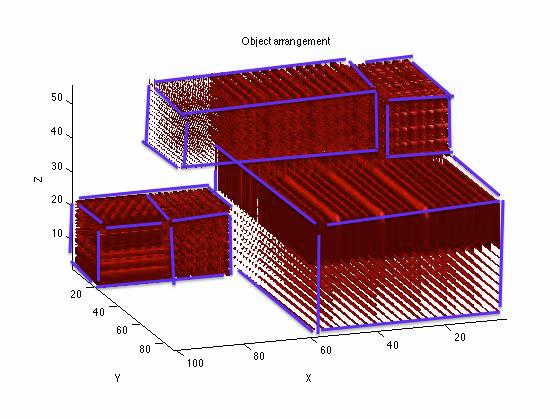
\includegraphics[width=0.45\textwidth]{packingExample.jpg}
    \caption{An example packing result, showing bounding boxes}
    \end{figure}

%------------------------------- Experimental Setup and Results ----------------------------------------
\section{Experiments}

\subsection{Experimental Setup}

To analyze the effectiveness of our pipeline, we run it from start to finish on images taken of a small plastic bowl and a macadamia nut cluster and compare how many macadamia nut clusters our algorithm can pack into the bowl compared to how many we can pack into the bowl manually. We seek to analyze how the number of clusters that can be packed into the bowl by our bin packing algorithm scales with the number of frames used to carve the bowl and the number of frames used to carve the macadamia nut cluster. 

Intuitively, as we add more frames to carve the bowl, we should be getting a progressively tighter upper bound on the actual expanse of the bowl, so increasing the number of frames used to carve the bowl should decrease strictly (assuming we are only adding frames, not removing and adding) decrease the number of clusters that we can pack. On the other hand, increasing the number of frames used to carve the nut cluster should also progressively slim the output voxel carving to the expanse of the real cluster, so using more frames to carve the nut cluster should strictly increase the number of clusters that our algorithm can fit into the bowl.

We began with 20 images of the macadamia nut cluster and 16 images of the small bowl, all with the calibration grid in the background. The camera angles are distributed roughly evenly on a spherical cap around the object (our rig involved mounting the object on a small pole that extended about a foot from a wall, so we were obstructed by the wall from taking pictures from the reverse). We construct silhouettes of the respective object from all images and store them. Then, to find the number of objects that we can pack using carvings formed from $n$ frames of the bowl and $m$ frames of the nut cluster, we sample as follows:

\begin{algorithmic}
\Function{MeanNumberPackings}{$c_0, iters, f_n, f_b$} \\

    \Comment{$c_0$ is the initial voxel box} \\ 
    \Comment{$f_n$ is an array containing the frames (silhouettes and camera parameters) of the cluster} \\
    \Comment{$f_b$ is an array containing the frames (silhouettes and camera parameters) of the bowl}
    
    \State $packings \gets 0$
    \For {$iter \in [1, iters]$}
        \State {$c_n \gets c_0$}
        \State {$c_b \gets c_0$}
        \For {$i \in \Call{SampleW/OReplacement}{20, m}$}
            \State {$c_n \gets \Call{Carve}{c_n, f_n (i)}$}
        \EndFor
        \For {$i \in \Call{SampleW/OReplacement}{16, n}$}
            \State {$c_b \gets \Call{Carve}{c_b, f_b (i)}$}
        \EndFor
        \State $packings \mathrel{+}= \Call{NumPackings}{c_b, c_n}$
    \EndFor
    
    \State \Return $packings/iters$
\EndFunction
\end{algorithmic}

\subsection{Results}
\begin{figure*}
    \centering
    \begin{subfigure}[t]{0.3\textwidth}
        \centering
        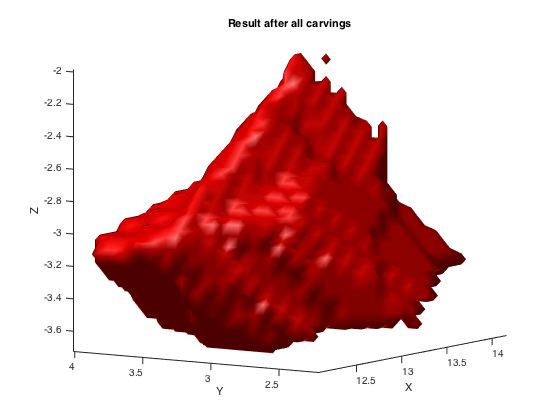
\includegraphics[width=\textwidth]{macadamia_4.png}
        \caption{Example carving of the macadamia nut cluster using four frames}
    \end{subfigure}
    ~ 
    \begin{subfigure}[t]{0.3\textwidth}
        \centering
        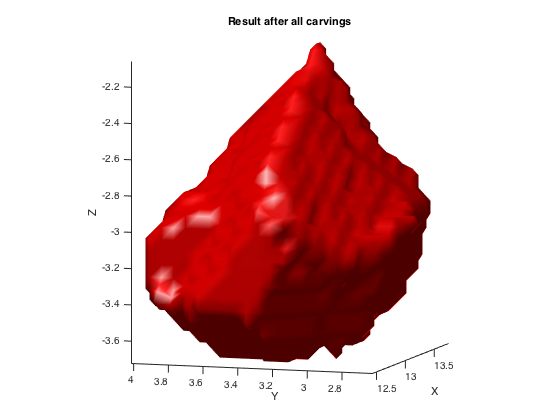
\includegraphics[width=\textwidth]{macadamia_8.png}
        \caption{Example carving of the macadamia nut cluster using eight frames}
    \end{subfigure}
    ~
    \begin{subfigure}[t]{0.3\textwidth}
        \centering
        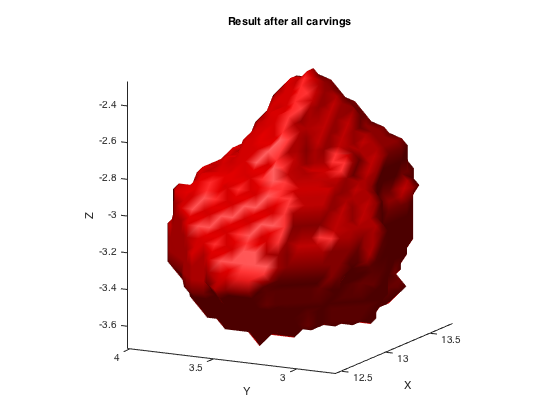
\includegraphics[width=\textwidth]{macadamia_14.png}
        \caption{Example carving of the macadamia nut cluster using fourteen frames}
    \end{subfigure}
    \caption{Carvings using sampled subset of images of macadamia nut cluster}
    \label{nut-carving}
\end{figure*}

\begin{figure*}
    \centering
    \begin{subfigure}[t]{0.3\textwidth}
        \centering
        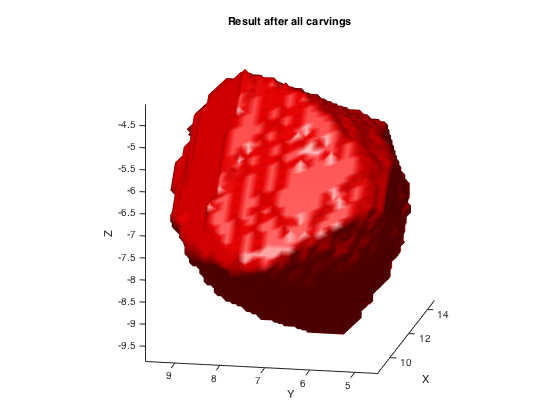
\includegraphics[width=\textwidth]{bluebowl2_4.png}
        \caption{Example carving of the small bowl using four frames}
    \end{subfigure}
    ~ 
    \begin{subfigure}[t]{0.3\textwidth}
        \centering
        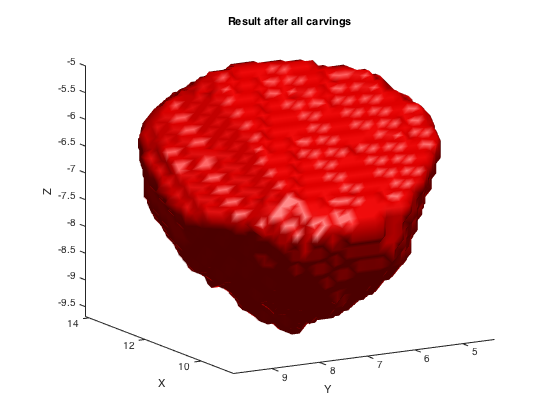
\includegraphics[width=\textwidth]{bluebowl2_8.png}
        \caption{Example carving of the small bowl using eight frames}
    \end{subfigure}
    ~
    \begin{subfigure}[t]{0.3\textwidth}
        \centering
        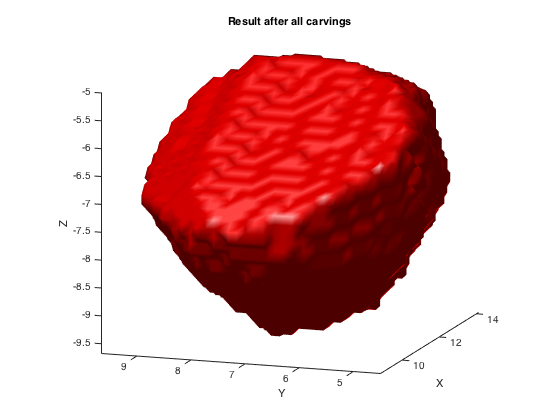
\includegraphics[width=\textwidth]{bluebowl2_12.png}
        \caption{Example carving of the small bowl using twelve frames}
    \end{subfigure}
    \caption{Carvings using sampled subset of images of small bowl}
    \label{bowl-carving}
\end{figure*}



Figure \ref{nut-carving} shows a sample progression of the carving as we use successively more frames to carve the cluster. Of particular note is that for a low number of frames, the oblong protrusion along the top of the cluster is especially large and the base of the cluster is broader and flatter than it is in reality. Figure \ref{nut-voxels} shows the effect on the volume that using additional frames has on the number of voxels: moving from four to eight frames eliminates over a quarter of the voxels used for the cluster. The effect on the deformations of adding the frames is demonstrated visually in figure \ref{nut-carving}: adding the additional frames substantially smooths out the base and shaves away the protrusion along the top.

\begin{figure}[H]
    \centering
    \begin{tabular}{|c|c|}
    \hline
    Number of sampled frames & Mean number of voxels \\
    \hline
    4 & 3982.8 \\
    8 & 2909 \\
    14 & 2285 \\
    \hline
    \end{tabular}
    \caption{Voxels as we vary the number of frames used to form the carving for the macadamia nut cluster}
    \label{nut-voxels}
\end{figure}

We should expect that refining these protrusions would have an out-sized impact on the number of objects that we are able to pack using our bin packing algorithm since we effectively consider the bounds of the object to be its extent in any direction. This effect can be seen in figure \ref{conts-objs}: as we increase the number of frames used to carve the macadamia nut cluster, the number of clusters that we can fit in the bowl increases without clear diminishing gains regardless of the number of frames used to carve the bowl.

\begin{figure}[H]
    \centering
    \begin{tabular}{|c|ccc|}
        \hline
           & 4    & 8    & 12 \\
        \hline
        4  & 2.38 & 1.58 & 1.58 \\
        8  & 2.88 & 2.33 & 2.08 \\
        14 & 3.50 & 3.17 & 2.67 \\
        \hline
    \end{tabular}
    \caption{Number of clusters that our algorithm is able to pack into the bowl. Number of frames used to carve bowl varies over columns, number of frames used to carve cluster varies over rows}
    \label{conts-objs}
\end{figure}

We can contrast with the effect that using more frames to carve the bowl has on the number of objects that we are able to pack into the bowl. Looking at figure \ref{conts-objs}, when using four or eight frames to carve the cluster, there is a clear limit to the gains (i.e. decrease in clusters packed) made from using additional frames to carve the bowl. This can largely be accounted for by the simplicity and lack of deformations present in the bowl. Looking at figure \ref{bowl-carving}, we see that the carving produced by using twelve frames is nearly identical to that produced by using eight frames. There simply are not any interesting features on the bowl that necessitate the use of additional frames to get a proper carving of. This is reflected in figure \ref{bowl-voxels}: Adding additional frames only slightly reduces the number of voxels that we use to represent the bowl. \\
\\It is also a noteworthy result that our silhouetting algorithm never caused a failure of the voxel carving method by not marking enough of a picture as part of the object, regardless of the number of frames used.

\begin{figure}[H]
    \centering
    \begin{tabular}[\textwidth]{|c|c|}
    \hline
    Number of sampled frames & Mean number of voxels \\
    \hline
    4 & 6250.3 \\
    8 & 5677 \\
    12 & 5320 \\
    \hline
    \end{tabular}
    \caption{Voxels as we vary the number of frames used to form the carving for the bowl}
    \label{bowl-voxels}
\end{figure}

%--------------------------------------------- Conclusion ------------------------------------------
\pagebreak
\section{Conclusions}

We create a semi-supervised system that uses photographs of objects and containers and determines how many objects can be packed.

First we use a calibration target in each photograph to determine camera parameters. Then by using K-Means in the CIELab color-space without lightness values, we create very robust silhouettes that are improved by infilling. From these silhouettes we use voxel carving to create a 3D model that is iteratively improved. Lastly we use a simple bounding-box method to greedily pack the 3D models of the objects inside the container.

We found that more complex objects such as the macadamia nut cluster require more photos to create a tight model while simple objects like the bowl show that there are diminishing returns from more photos of the object.

Future work could greatly improve usability of the system by providing a GUI to select the color of object to be silhouetted, or even have the program determine which cluster to use automatically. Ideally, the method would be made to not require the calibration checkerboard or necessitate the user taking lots of photos. Also, the bin packing system can be greatly improved to allow for rotations of objects in the containers as well. If it is improved to allow for objects' concavities to intersect, then perhaps voxel carving will be too simple of a method to generate the 3D models.


{\small
\bibliographystyle{ieee}
\bibliography{sources.bib}
}

\end{document}
